
\documentclass[tikz,border=2mm]{standalone}
\usepackage{tikz}
\usetikzlibrary{shapes,arrows,positioning,automata,shadows}
\begin{document}
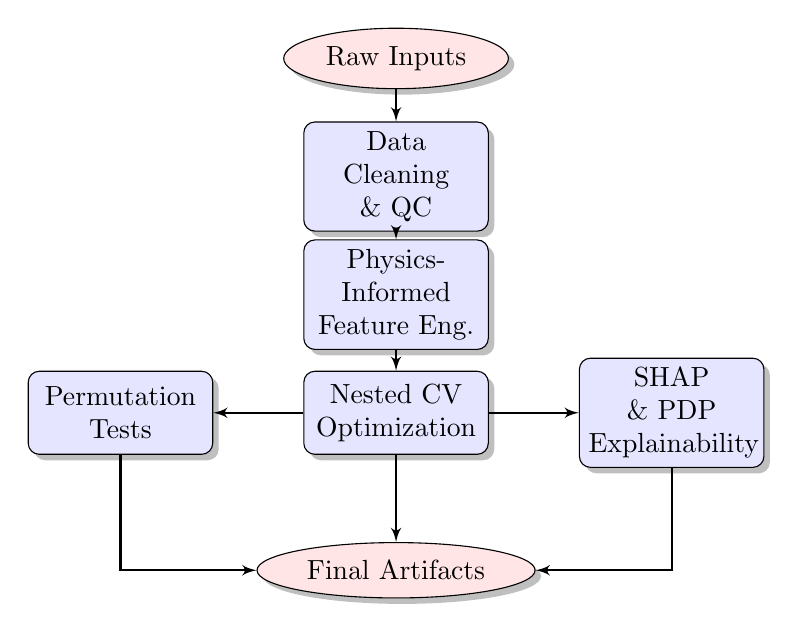
\begin{tikzpicture}[
    node distance=1.5cm,
    auto,
    block/.style={rectangle, draw, fill=blue!10, text width=6em, text centered, rounded corners, minimum height=3em, drop shadow},
    cloud/.style={draw, ellipse, fill=red!10, node distance=2cm, minimum height=2em, drop shadow},
    line/.style={draw, -latex', thick}
]
    % Nodes
    \node [cloud] (start) {Raw Inputs};
    \node [block, below of=start] (prep) {Data Cleaning \\ \& QC};
    \node [block, below of=prep] (feat) {Physics-Informed \\ Feature Eng.};
    \node [block, below of=feat] (model) {Nested CV \\ Optimization};
    \node [block, left of=model, node distance=3.5cm] (perm) {Permutation \\ Tests};
    \node [block, right of=model, node distance=3.5cm] (expl) {SHAP \& PDP \\ Explainability};
    \node [cloud, below of=model] (end) {Final Artifacts};

    % Paths
    \path [line] (start) -- (prep);
    \path [line] (prep) -- (feat);
    \path [line] (feat) -- (model);
    \path [line] (model) -- (end);
    \path [line] (model) -- (perm);
    \path [line] (model) -- (expl);
    \path [line] (perm) |- (end);
    \path [line] (expl) |- (end);

\end{tikzpicture}
\end{document}
        